% Created 2021-10-06 Wed 13:57
% Intended LaTeX compiler: pdflatex
\documentclass[11pt]{article}
\usepackage[utf8]{inputenc}
\usepackage[T1]{fontenc}
\usepackage{graphicx}
\usepackage{grffile}
\usepackage{longtable}
\usepackage{wrapfig}
\usepackage{rotating}
\usepackage[normalem]{ulem}
\usepackage{amsmath}
\usepackage{textcomp}
\usepackage{amssymb}
\usepackage{capt-of}
\usepackage{hyperref}
\author{Tomaz Geddes de Almeida}
\date{\today}
\title{Geography Extension Task}
\hypersetup{
 pdfauthor={Tomaz Geddes de Almeida},
 pdftitle={Geography Extension Task},
 pdfkeywords={},
 pdfsubject={},
 pdfcreator={Emacs 27.2 (Org mode 9.4.4)}, 
 pdflang={English}}
\begin{document}

\maketitle
\tableofcontents


\section{References}
\label{sec:orgb141844}

\href{https://www.countryfile.com/go-outdoors/days-out/britains-best-coastal-caves-arches-and-stacks/}{Britain’s best coastal caves, arches and stacks}

\href{http://mapapps.bgs.ac.uk/geologyofbritain/home.html}{Geology Finder}

\section{Fingal's Cave}
\label{sec:org6aadb39}

\subsection{Map}
\label{sec:orgd535c53}
\begin{center}
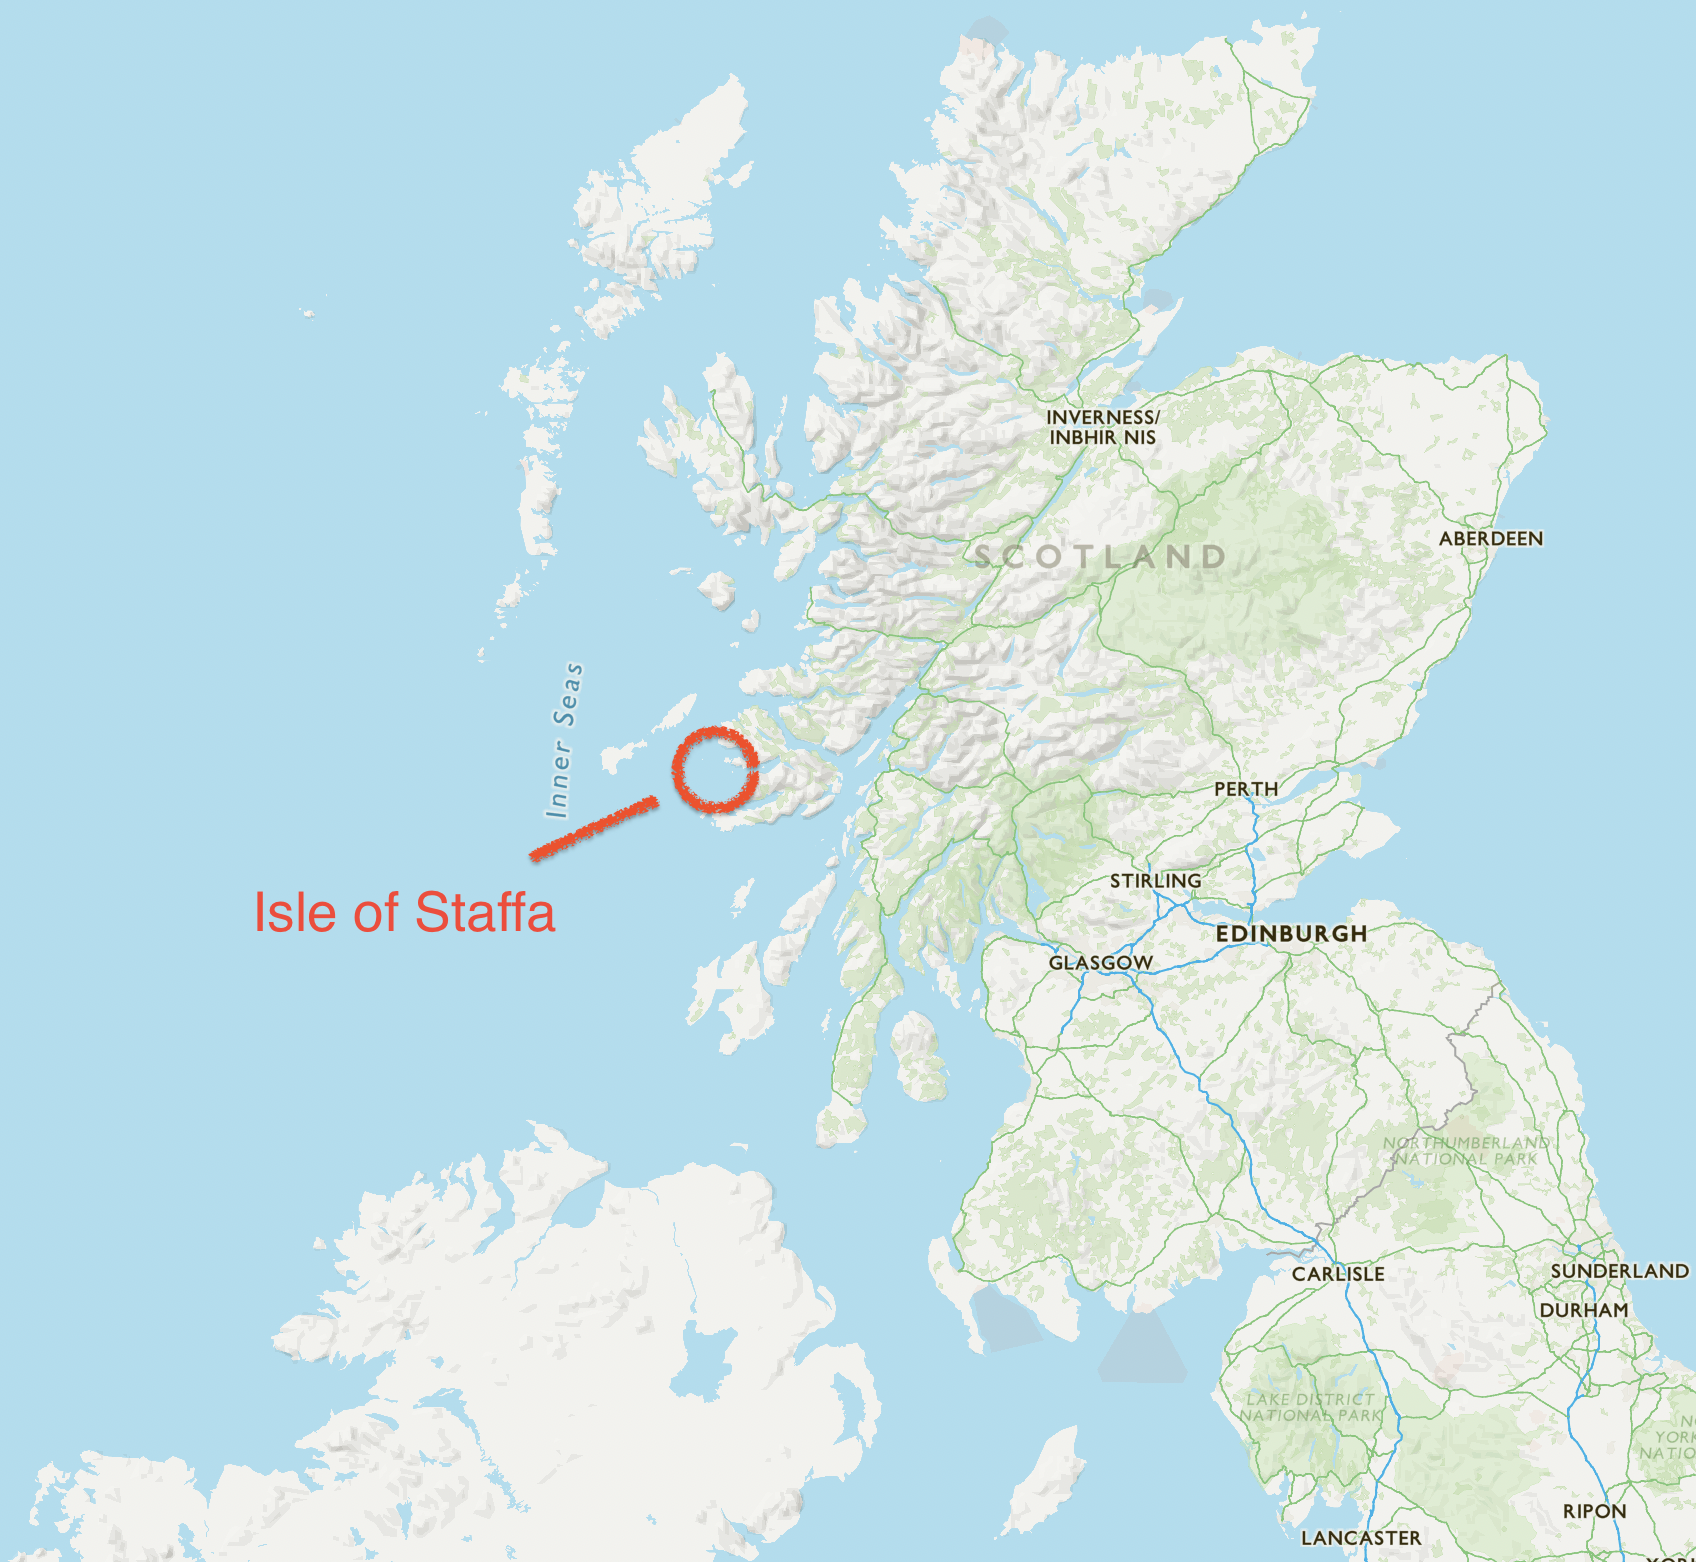
\includegraphics[width=.9\linewidth]{Images/isle-of-staffa.png}
\end{center}

\subsection{Image}
\label{sec:orgccfa781}
\begin{center}
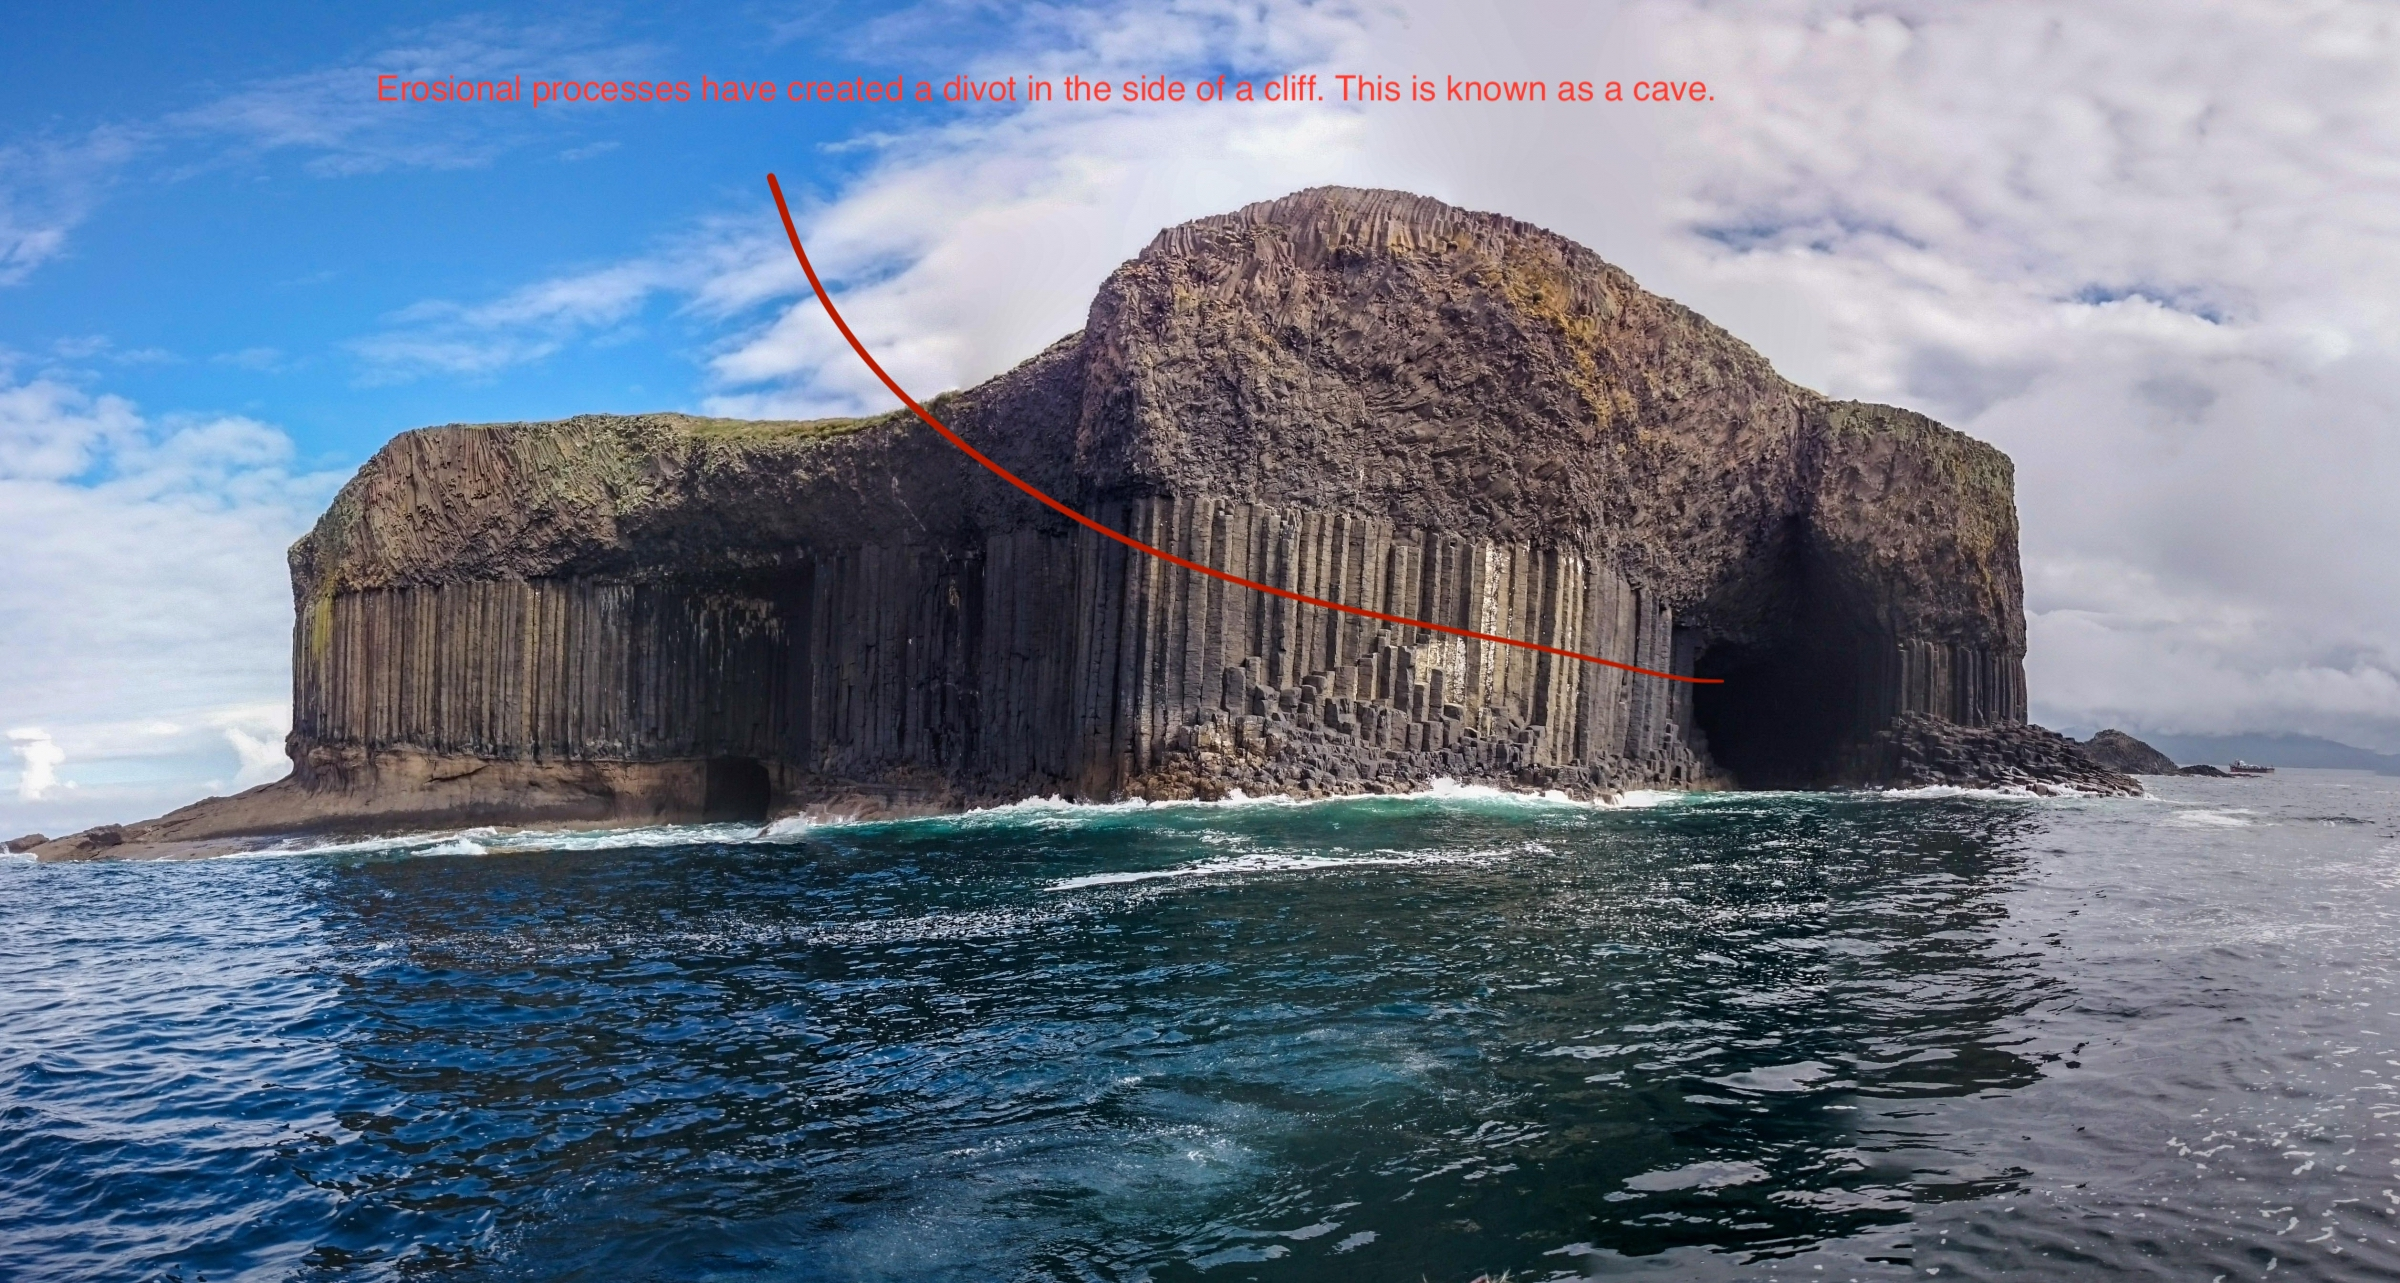
\includegraphics[width=.9\linewidth]{Images/cave-image.jpg}
\end{center}

\subsection{Description}
\label{sec:orge3a5b7b}

\begin{itemize}
\item Geology 

\begin{itemize}
\item \emph{Mull Lava Group - Basalt. Igneous Bedrock formed approximately 56 to 66 million years ago in the Palaeogene Period. Local environment previously dominated by eruptions of silica-poor magma.}

\item \emph{These igneous rocks are volcanic (extrusive) in origin. Poor in silica, they form fluid flows of lava with feeder dykes and sills.}
\end{itemize}

\item Fingal's cave is located on the Isle of Staffa off the west coast of Scotland. It is composed of regular basalt columns on the lower half of the cliff face.
\end{itemize}

\section{Black Church Rock}
\label{sec:org928d6f2}
\subsection{Map}
\label{sec:org02db919}
\begin{center}
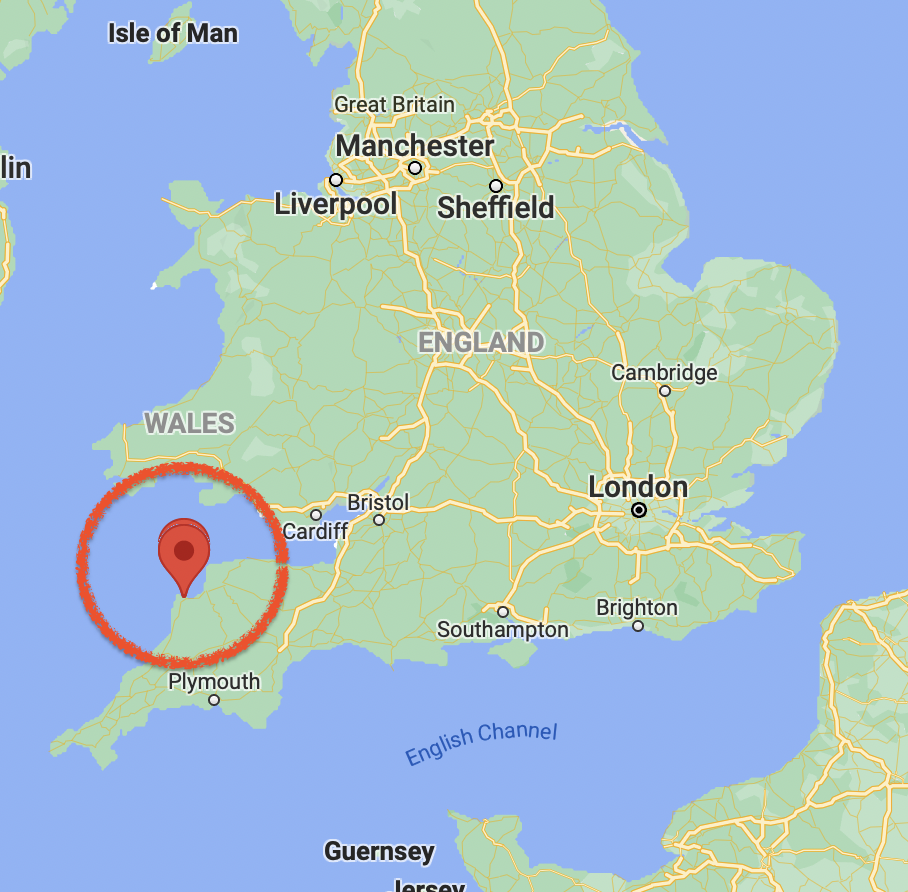
\includegraphics[width=.9\linewidth]{Images/black-church-rock.png}
\end{center}

\subsection{Image}
\label{sec:org9bc6478}
\begin{center}
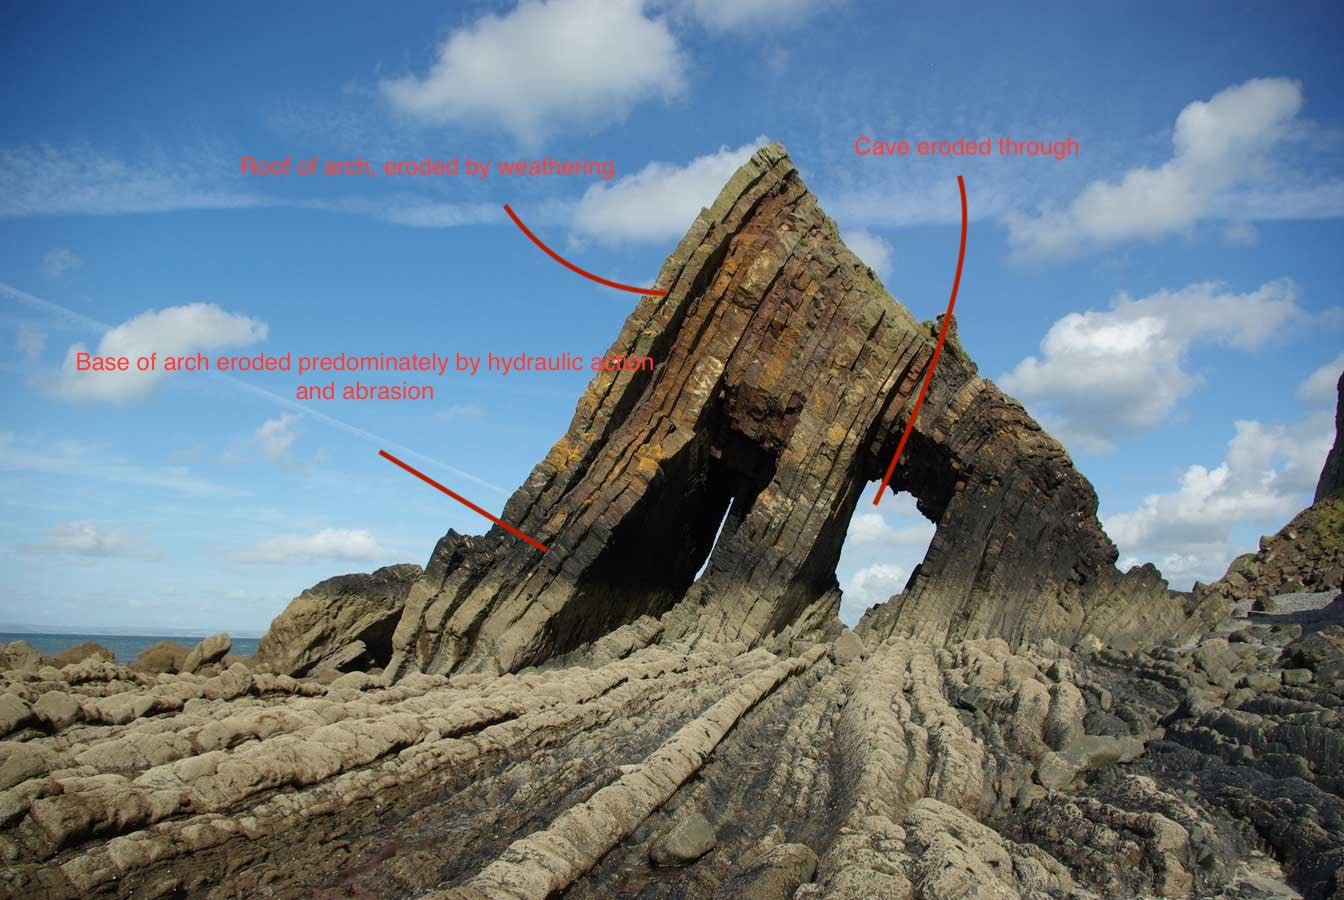
\includegraphics[width=.9\linewidth]{Images/arch-image.jpg}
\end{center}

\subsection{Description}
\label{sec:org54ca3aa}

\begin{itemize}
\item Geology 

\begin{itemize}
\item \emph{Mudstone, Siltstone And Sandstone. Sedimentary Bedrock formed approximately 309 to 326 million years ago in the Carboniferous Period}

\item \textbf{Setting:} \emph{sub-aqueous slopes.}
\end{itemize}

\item Black Church Rock is located one mile east of Brownsham car park on the north coast of Devon.
\end{itemize}

\section{Stacks of Dunscaby}
\label{sec:orga3eadb7}

\subsection{Map}
\label{sec:org049f76e}
\begin{center}
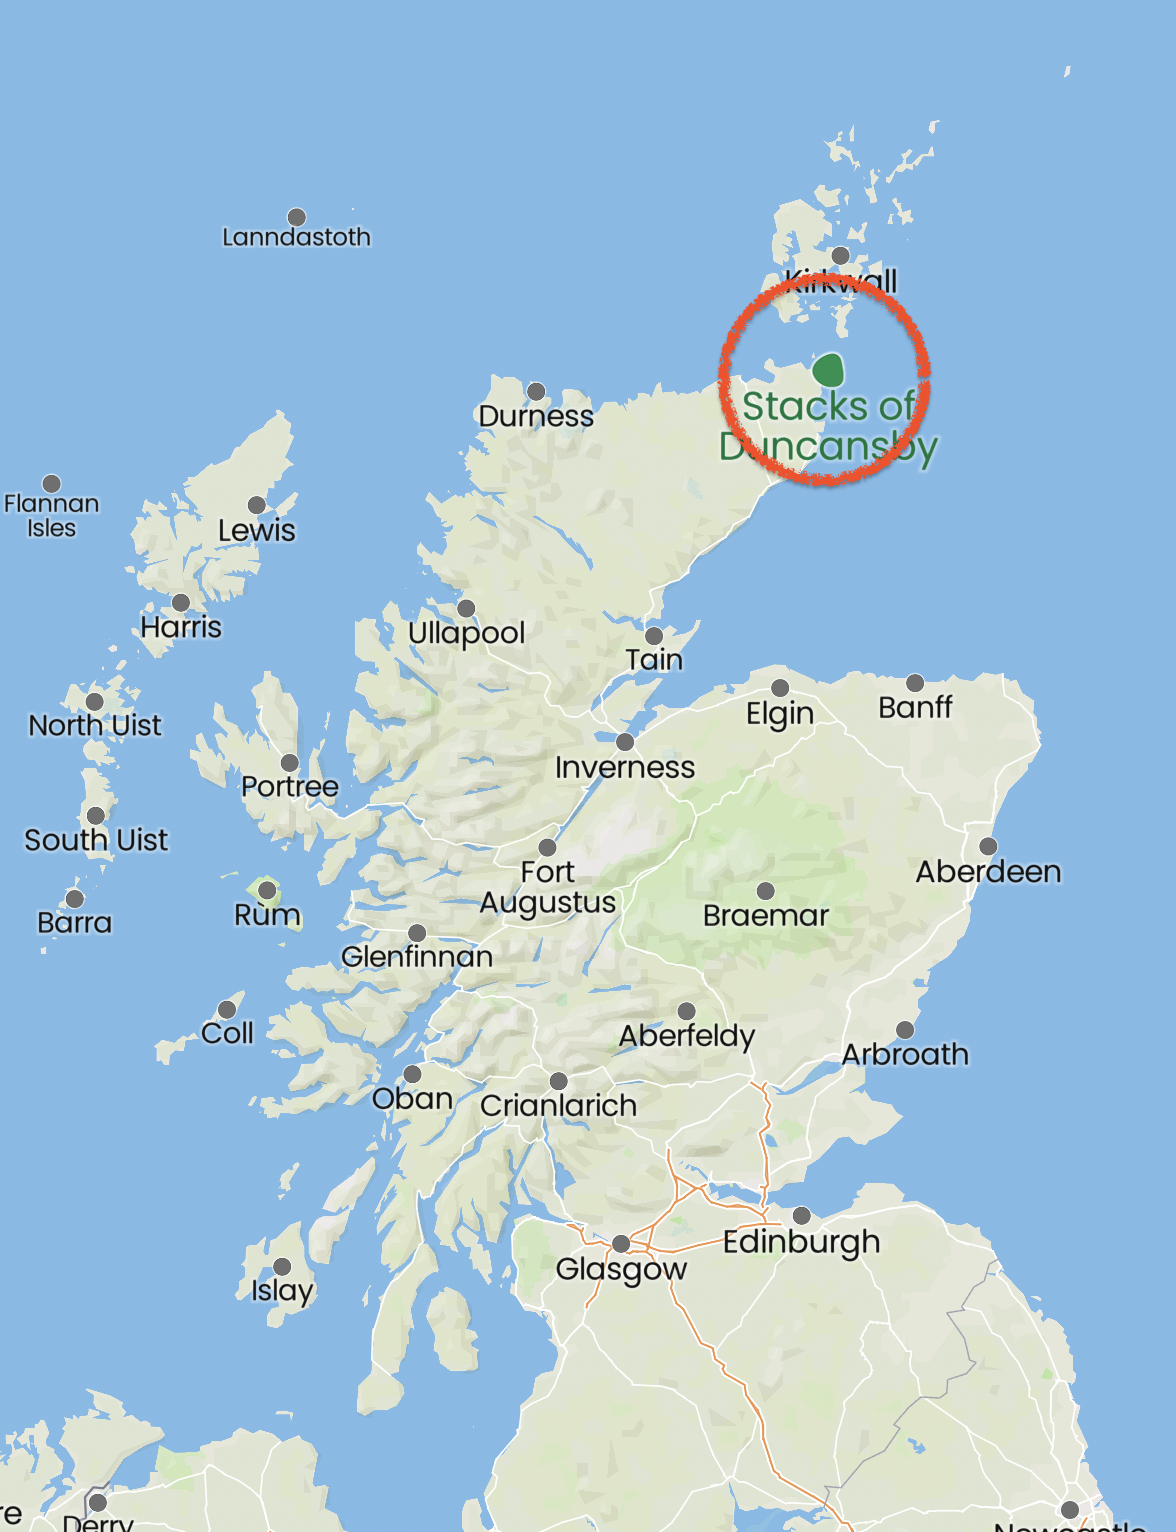
\includegraphics[width=.9\linewidth]{Images/stacks-of-dunscaby.png}
\end{center}

\subsection{Image}
\label{sec:orgc4ac43f}
\begin{center}
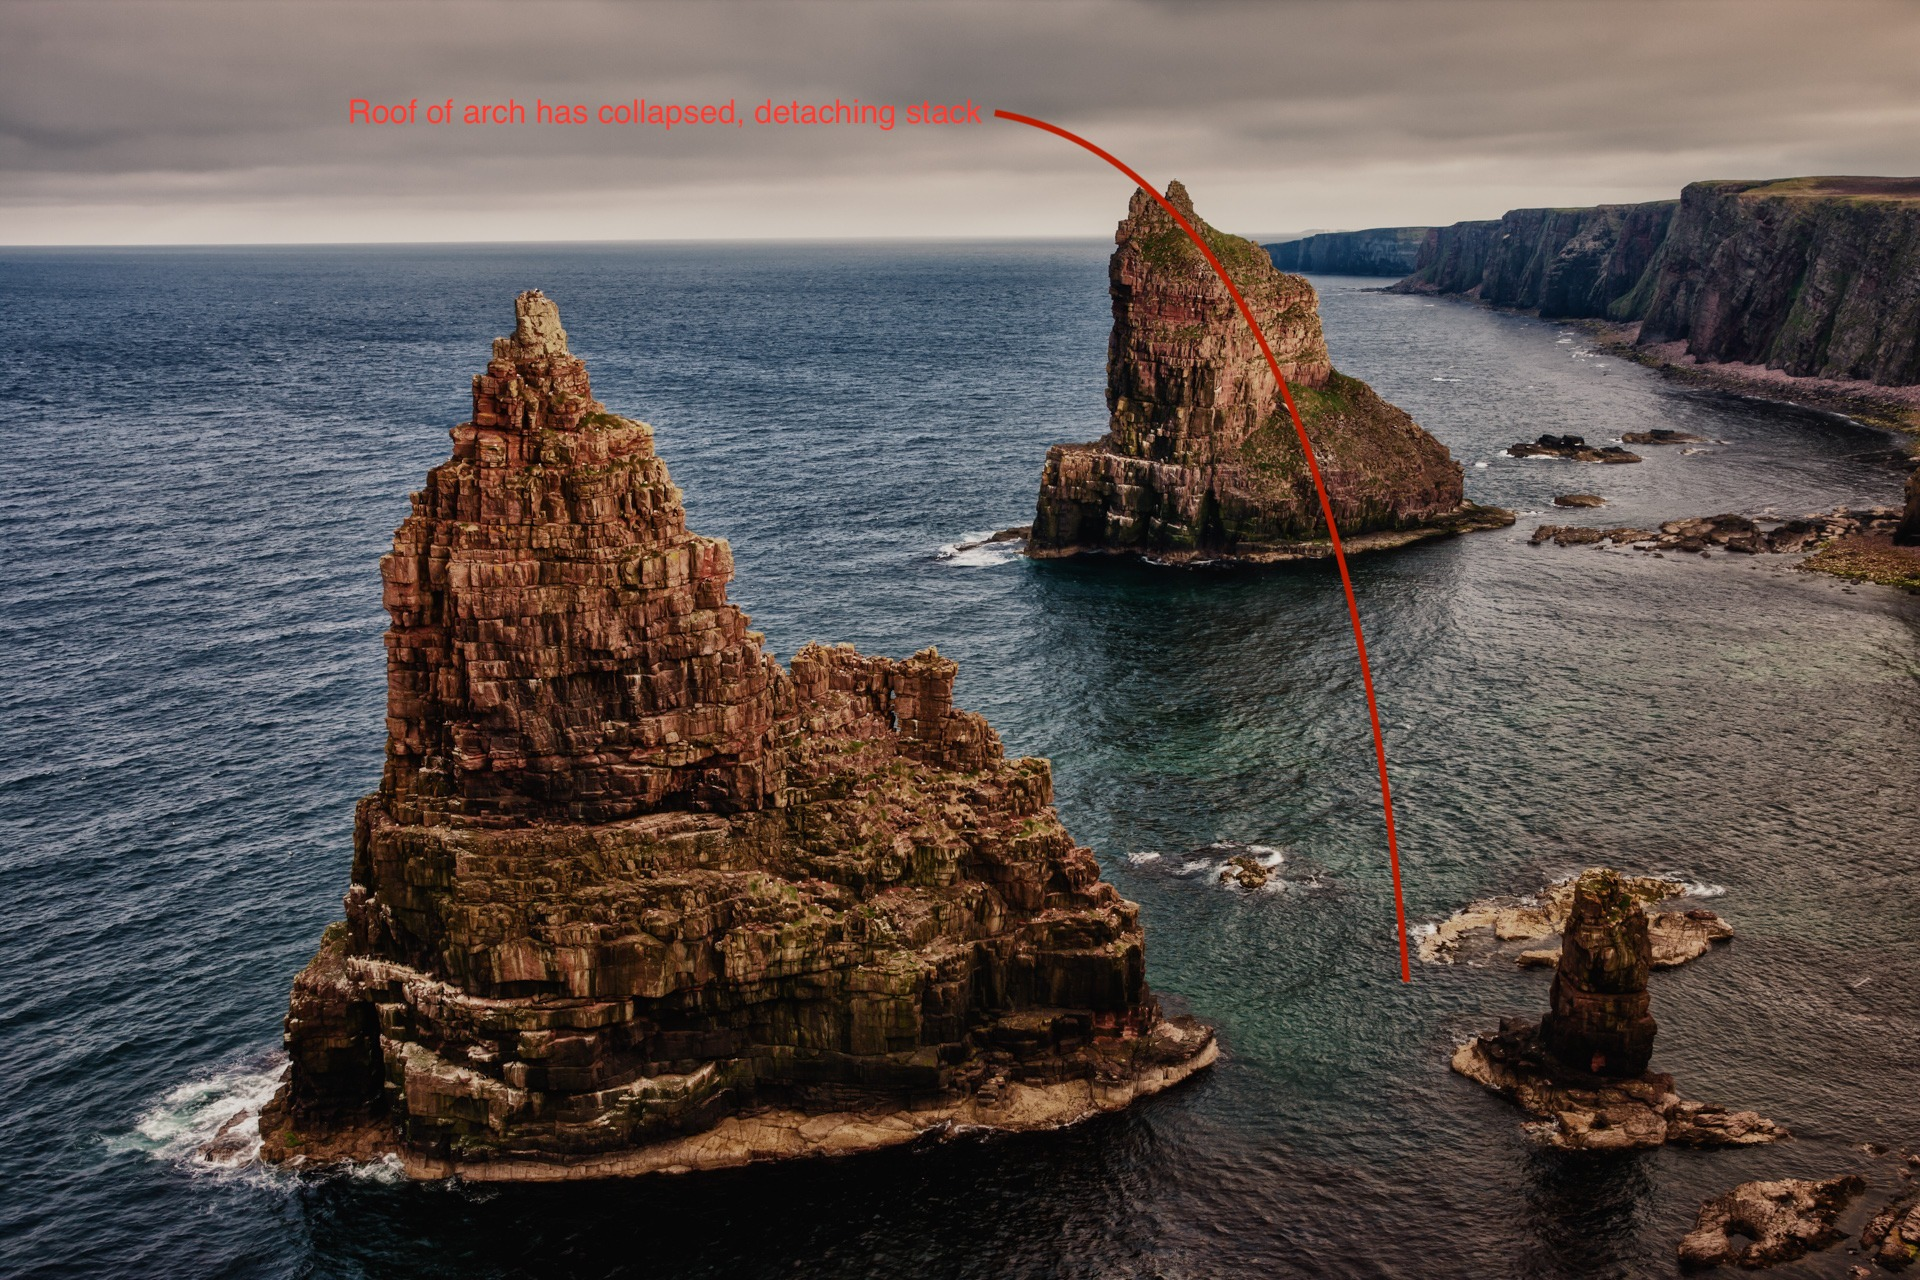
\includegraphics[width=.9\linewidth]{Images/stacks-image.jpg}
\end{center}

\subsection{Description}
\label{sec:org6415349}

\begin{itemize}
\item Geology

\begin{itemize}
\item \emph{Middle Old Red Sandstone (undifferentiated) - Conglomerate, Sandstone, Siltstone And Mudstone. Sedimentary Bedrock formed approximately 385 to 398 million years ago in the Devonian Period.}

\item \textbf{Setting} : \emph{rivers and alluvial fans.}
\end{itemize}

\item Stacks of Duncansby, Scotland

The Stacks of Dunscaby are located on the north-east coast of Scotland.
\end{itemize}

\section{Formation of Caves, Arches, Stacks Stumps}
\label{sec:orgc4625c6}
\subsection{Caves}
\label{sec:orgd6c112a}
(Dictionary) \emph{A natural underground chamber in a hillside or cliff} . Essentially, a cave is the first landform created when coastal erosion acts on a cliff.   

Lines of weakness in a headland are especially vulnerable to erosion. Coastal erosion, predominately hydraulic action and abrasion, act on these fault lines until a cave is formed.

\subsection{Arches}
\label{sec:orgbdb2cff}
If a cave is situated on one side of a headland, it could be eroded through to form an arch.

\subsection{Stacks}
\label{sec:org7b90546}
Continued erosion by  the sea widens the arch. As the base of the arch shrinks due to erosional processes such as hydraulic action more pressure is placed on the roof. Eventually, the roof collapses, leaving a stack.

\subsection{Stumps}
\label{sec:org6ceae8a}
Further erosion and weathering over time causes the stack to collapse, leaving a stump.

\section{Formation of Wave Cut Platforms}
\label{sec:org8c81b46}

When waves break against a cliff, erosional processes operating close to the high-tide line takes a 'bite' out of the base of the cliff - a notch. These processes include hydraulic action, whereby gaps in the rock face are compressed by waves acting on the coast, and abrasion.  As the notch gets deeper, often over a period of many years, the overhanging rock can no longer support its own weight and so collapses, causing the cliff to retreat. In its place, the retreating cliffs leave a gently sloping rocky platform called a wave-cut platform. Wave-cut platforms are often smoothed by abrasion. Eventually, constructive waves may deposit sediment on such a platform to form a beach.
\end{document}
